%% Chapter 5 %%%
\chapter[Ошибка базовой оценки]{\emph{Р}-значение и ошибка базовой оценки}
\label{chp5}
\chaptermark{Ошибка базовой оценки}

Как вы уже видели, \emph{р}-значения интерпретировать непросто. То, что мы получили статистически незначимые результаты, не означает, что различий не существует. А что означает статистически значимый результат?

Давайте посмотрим на примере. Предположим, я решил протестировать сотню потенциальных лекарств от рака. Только десять из них реально действуют, но я не знаю, какие именно - мне нужно проводить эксперименты, чтобы определить это. В самих экспериментах, я буду ориентироваться на $p<0,05$ в оценке различий с действием плацебо, что будет демонстрировать полезность тестируемого лекарства. 

Для иллюстрации, на изображении ниже каждая клетка таблицы представляет собой одно лекарство. Синим отмечены те клетки, которые соответствуют действующим лекарствам:


%\newpage % делаем разрыв, чтобы картинка была первой на след странице

%%%%%%%%%%%%%% figure 5 %%%%%%%%%%%%%%%%%%5
\begin{figure}[h!]
    \centering
    
\includegraphics[width=0.4\textwidth]{drug-grids-1}
    %\caption{}
    \label{fig5:drug-grid-1}
\end{figure}
%%%%%%%%%%%%%%% end of figure 5 %%%%%%%%%%%%%%%%%%%

Как мы видили ранее, в большинстве испытаний сложно определить каждое хорошее лекарство. Давайте предположим, что статистическая мощность моих тестов - 0,8. Из десяти действующих лекарств, я смогу правильно распознать примерно 8 (отмечены фиолетовым на иллюстрации ниже):

\newpage % делаем разрыв, чтобы картинка была первой на след странице

%%%%%%%%%%%%%% figure 6 %%%%%%%%%%%%%%%%%%5
\begin{figure}[h!]
    \centering
    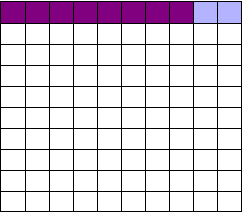
\includegraphics[width=0.4\textwidth]{drug-grids-2}
    %\caption{}
    \label{fig5:drug-grid-2}
\end{figure}
%%%%%%%%%%%%%%% end of figure %%%%%%%%%%%%%%%%%%%


Я также предположу, что около 5 из 90 недействующих лекарств будут иметь значимые эффекты. Почему? Напомню, что \emph{p}-значение подсчитывается исходя из предположения об отсутствии эффекта, т.е. $ p =0,05$ означает, что существует 5\% шанс сделать ошибочный вывод о том, что недействующее лекарство на самом деле действует.

Таким образом, я провожу свои эксперименты и делаю вывод о том, что у меня есть 13 действующих лекарств: 8 хороших лекарств и 5 тех, что я мог ошибочно включить в свой список (показаны красным на илюстрации ниже):


%\newpage % делаем разрыв, чтобы картинка была первой на след странице

%%%%%%%%%%%%%% figure 6 %%%%%%%%%%%%%%%%%%5
\begin{figure}[h!]
    \centering
    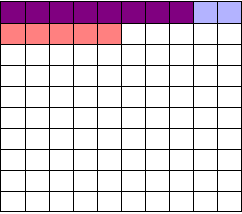
\includegraphics[width=0.4\textwidth]{drug-grids-3}
    %\caption{}
    \label{fig5:drug-grid-3}
\end{figure}
%%%%%%%%%%%%%%% end of figure %%%%%%%%%%%%%%%%%%%

Шанс того, что любое из ``действующих'' лекарств будет действительно эффективным, составляет только 6\%. Если бы я случайным образом выбрал одно лекарство из ста, провёл на нем свои тесты и обнаружил бы статистически значимую связь на уровне $p<0,05$, то существует всего 62\% шанса на то, что это лекарство действительно эффективно. Говоря терминами статистики, мои шансы совершить ошибку первого рода (оценка ложной тревоги) - это доля ложных положительных результатов в общем количестве статистически значимых результатов - составляют 38\%.  

Поскольку базовая оценка эффективности лекарств от рака довольно низкая - только около 10\% от множественных испытаний и лекарств дают какой-то результат, - большинство из тестируемых лекарств не действуют, и мы становимся особенно уязвимы к совершению ошибки первого рода. Будь я полным неудачником и будь у меня хоть целый грузовик совершенно бесполезных лекарств, базовая оценка эффективности которых составляет 0\%, я бы имел 0\% шанса на получение хоть какого-либо статистически значимого результата. Тем не менее, я все равно получу результат в $p<0,05$ для 5\% этих лекарств.

Часто можно слышать, как люди приводят в пример \emph{p}-значения в качестве показателя малой вероятности получения ошибки. ``Существует только 1 шанс из 10000, что такой результат возник случайным образом'' - говорят они, потому что получили значение $p=0,0001$. Увы, нет! Такое утверждение игнорирует базовую оценку, и встречается под названием \emph{ошибка базовой оценки}. Напомним, как определяется \emph{p}-значение:

\begin{quotation}

\textbf{\emph{P}-значение} можно определить как вероятность получить результат равный или больший, чем в реальности наблюдаемый, при условии, что никакого эффекта или различий обнаружено не было (нулевая гипотеза).   

\end{quotation}


\emph{P}-значение рассчитывается, основываясь на предположении о том, что лекарство \emph{не действует}, и даёт нам вероятность получения данных равных или больше тех, что мы получили. Оно не даёт нам вероятность того, что лекарство действует.

Когда кто-либо использует полученные \emph{p}-значения в качестве доказательства того, что они правы, запомните это. Вероятность ошибки их исследования, скорее всего, довольно высока. В сферах, где большинство проверяемых гипотез опровергаются, как, например, в первичных тестах лекарств (большинство таких лекарств не проходят тесты), вполне вероятно, что большинство ``статистически значимых'' результатов с $p < 0,05$ на самом деле всего лишь случайность.

Отличный пример тому - тесты на медицинскую диагностику.


\section[В медицинских испытаниях]{Ошибка базовой оценки в медицинских испытаниях}
\label{chp5:base-rateF}
\sectionmark{Медицинские испытания}

Существуют некоторые разногласия во мнениях по поводу использования маммографии при тестировании на рак груди. Некоторые считают, что опасность получить ложноположительный результат (и последующие ненужные биопсия, хирургическое вмешательство и химиотерапия) превышает те преимущества, которые даёт раннее обнаружение рака. Это статистический вопрос, давайте попробуем дать оценку.

Предположим, что у 0,8\% женщин, которым предписали маммографию, действительно  рак груди. У 90\% женщин, имеющих рак груди, маммография сможет его обнаружить. (Это статистическая мощность теста, но приблизительная, поскольку очень сложно сказать, сколько случаев рака груди мы упустили, если мы не знаем, что они вообще есть.) Тем не менее, из женщин, не имеющих рака груди, около 7\% получат ложноположительный результат на маммографии, ведущий к дальнейшим тестам, лечению и биопсии. Если вы получили положительный результат маммографии, каковы шансы на то, что у вас действительно рак груди?

Опуская те ситуации, когда ты, читатель, мужчина\footnote{Забавно, но если вы - мужчина, это не исключает возможности получить рак груди; это лишь делает вероятность чрезвычайно малой.}, ответ - 9\%.\cite{kramer_how_2005}

Несмотря на то, что тест даёт ложноположительный результат лишь у 7\% женщин, не имеющих рак груди, что аналогично $p < 0,07$, порядка 91\% положительных результатов на самом деле ложноположительные.

Как я это рассчитал? Точно таким же методом, как и в примере про лекарство от рака. Представьте себе 1000 случайно выбранных женщин, которые решили пройти маммографию. У восьми из них (0,8\%) есть рак груди. Маммография обнаруживает правильно около 90\% случаев рака, т.е. примерно у семи из восьми женщинрак будет обнаружен. Однако, остается 992 женщины без рака груди, и 7\% из них получат ложноположительный результат, т.е. у 70 женщин будет неверно диагностирован рак груди.

В сумме у нас получается 77 женщин с положительным результатом маммографии, у 7 из которых действительно есть рак груди. Только у 9\% женщин с положительным результатом по маммографии действительно есть рак груди.

Если задать этот вопрос студентам, изучающим статистику, и преподавателям научной методологи, более трети из них не смогут ответить верно.\cite{kramer_how_2005} Если задать его врачам, две трети из них провалятся на этом вопросе.\cite{bramwell_health_2006} Они ошибочно делают вывод о том, что $p < 0,05$ означает 95\% вероятность того, что результат истинный, хотя, как вы можете видеть из приведённых примеров, вероятность того, что положительный результат истиннен, зависит от того, какая часть проверенных гипотез верна. И нам просто повезло, что в любой момент времени рак груди возникает лишь у небольшой части женщин. 

Пролистайте вводные учебники по статистике и вы встретите подобное заблуждение довольно часто. \emph{P}-значения трудны для понимания, а ошибка базовой оценки встречается повсеместно.  


\section{Оружие против ошибки базовой оценки}
\label{chp5:arms-baserateF}
\sectionmark{Оружие против ошибки базовой оценки}

Чтобы столкнуться с этой ошибкой, нет нужды проводить расширенное исследование или тестировани на рак. А что, если вы делаете социологическое исследование? Например, вы хотите опросить американцев, чтобы узнать как часто они используют оружие в целях самообороны. В конце концов, в основе аргументов сторонников контроля оружия находится именно право на самозащиту, поэтому важно определить, используется ли оружие в большинстве случаев для защиты и перевешивает ли это недостатки, например, убийства.

Один из способов собрать необходимые данные - опрос. Можно опросить репрезентативную выборку американцев, узнав, владеют ли они оружием, и если да, использовали ли когда-нибудь оружие для защиты своего дома от незаконного проникновения или для защиты себя от ограбления. Затем можно сравнить полученные данные со статистикой правоохранительных органов об использовании оружия в случаях убийства и сделать вывод на основании этого вывод.

Такие опросы уже проводились, и результаты их довольно интересные. Один телефонный опрос, проведенный в 1992 году, позволил оценить, что американские граждане используют оружие в целях самообороны до 2,5 миллиона раз ежегодно - то есть, около 1\% американских взрослых защищали себя с помощью оружия. В 34\% случаях это была защита от незаконного проникновения в жилище, т.е. порядка 845000 взломов было остановлено владельцами оружия. Но за 1992 год было совершено только 1,3 миллиона взломов в дома, в которых кто-либо был. Две трети из них произошли в тот момент, когда жильцы дома спали, и сам факт взлома и ограбления был обнаружен уже после того, как воры покинули жилище. Получается, что остается порядка 430000 случаев взлома, когда домовладельцы были в доме и противостояли грабителям и, как нас пытаются убедить, в 845000 случаях из них, грабители были остановлены жителями - владельцами оружия.\cite{hemenway_survey_1996}   


Ой!


Что произошло? Почему опрос переоценил количество случаев использования оружия в целях самозащиты? По тем же причинам, что и маммография давала завышенную оценку случаев рака груди: гораздо больше возможностей для ложноположительных результатов, чем ложноотрицательных. Если 99,9\% людей никогда не использовали оружие в целях самообороны, но 1\% из них ответит ``да'' на любой вопрос просто ради забавы, еще 1\% ответит так, чтобы выглядеть более мужественно, а 1\% просто неправильно поймёт вопрос, - вы получите значительную переоценку использования оружия в целях самозащиты.

А что насчет ложноотрицательных результатов? Могут ли они быть сбалансированы людьми, которые говорили ``нет'', даже если они лично застрелили грабителя на прошлой неделе? Ответ: нет. Если лишь немногие действительно используют оружие в качестве самообороны, тогда возможность получить ложноотрицательные результаты слишком низка. Они вытесняются ложноположительными результатами.

Эта ситуация аналогична примеру с лекарствами от рака, описанному ранее. Здесь \emph{p}-значение - это вероятность того, что кто-нибудь будет ошибочно утверждать, что он использовал оружие в целях самообороны. Даже если значение \emph{p} будет небольшим, ваш окончательный ответ будет все равно неверным. 


Чтобы снизить \emph{p}-значение, криминологи используют более детальные опросы. Например, в исследованиях показателя национальной виктимизации населения (NCVS) используются подробные сидячие интервью с исследователями, где респондентов спрашивают о деталях преступлений и использования ими оружия в целях самообороны. Чем больше подробностей в опросе, тем лучше исследователи могут оценить, подходит ли конкретный инцидент под критерии самообороны. Результаты таких исследований гораздо скромнее - около 65000 случаев в год. Существует вероятность того, что эта оценка занижена, но и меньший шанс массовой переоценки.     


\section[Не удалось в первый раз - пробуйте еще]{Не удалось в первый раз - пробуйте еще}
\label{chp5:try-again}

Ошибка базовой оценки показывает, что ложноположительные результаты более вероятны в том случае, если вы считаете $p < 0,05$ критерием значимости. Большинство современных исследований не полагается только на один показатель значимости - они сравнивают эффекты нескольких факторов, надеясь найти один с наиболее значимыми эффектами.

Например, представьте себе исследование, в котором проверялось бы, являются ли драже причиной появления угревой сыпи на коже, путём исследования эффекта драже различного цвета: %см. \hyperref[fig5:xkcd-significant]{комикс xkcd}.

\newpage % делаем разрыв, чтобы картинка была первой на след странице

%%%%%%%%%%%%%% figure 7 %%%%%%%%%%%%%%%%%%5
\begin{figure}[h!]
    \centering
    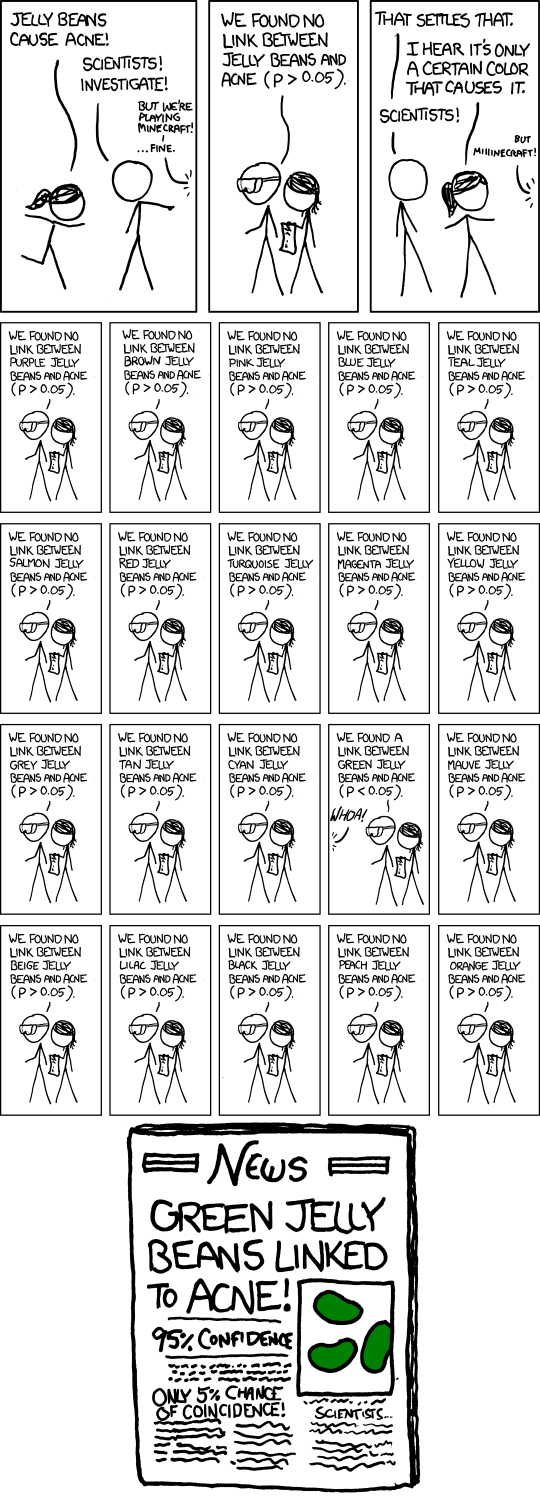
\includegraphics[width=0.5\textwidth]{xkcd-significant}
    \caption{xkcd-комикс, автор Randall Munroe. \href{http://xkcd.com/882/}{http://xkcd.com/882/}}
    \label{fig5:xkcd-significant}
\end{figure}
%%%%%%%%%%%%%%% end of figure %%%%%%%%%%%%%%%%%%%

As you can see, making multiple comparisons means multiple chances for a false positive. For example, if I test 20 jelly bean flavors which do not cause acne at all, and look for a correlation at p<0.05 significance, I have a 64\% chance of a false positive result.54 If I test 45 materials, the chance of false positive is as high as 90%.

It’s easy to make multiple comparisons, and it doesn’t have to be as obvious as testing twenty potential medicines. Track the symptoms of a dozen patients for a dozen weeks and test for significant benefits during any of those weeks: bam, that’s twelve comparisons. Check for the occurrence of twenty-three potential dangerous side effects: alas, you have sinned. Send out a ten-page survey asking about nuclear power plant proximity, milk consumption, age, number of male cousins, favorite pizza topping, current sock color, and a few dozen other factors for good measure, and you’ll find that something causes cancer. Ask enough questions and it’s inevitable.

A survey of medical trials in the 1980s found that the average trial made 30 therapeutic comparisons. In more than half of the trials, the researchers had made so many comparisons that a false positive was highly likely, and the statistically significant results they did report were cast into doubt: they may have found a statistically significant effect, but it could just have easily been a false positive.54

There exist techniques to correct for multiple comparisons. For example, the Bonferroni correction method says that if you make n comparisons in the trial, your criterion for significance should be p<0.05/n. This lowers the chances of a false positive to what you’d see from making only one comparison at p<0.05. However, as you can imagine, this reduces statistical power, since you’re demanding much stronger correlations before you conclude they’re statistically significant. It’s a difficult tradeoff, and tragically few papers even consider it.

\section{Red herrings in brain imaging}
\label{chp5:redherrings}

Neuroscientists do massive numbers of comparisons regularly. They often perform fMRI studies, where a three-dimensional image of the brain is taken before and after the subject performs some task. The images show blood flow in the brain, revealing which parts of the brain are most active when a person performs different tasks.

But how do you decide which regions of the brain are active during the task? A simple method is to divide the brain image into small cubes called voxels. A voxel in the “before” image is compared to the voxel in the “after” image, and if the difference in blood flow is significant, you conclude that part of the brain was involved in the task. Trouble is, there are thousands of voxels to compare and many opportunities for false positives.

One study, for instance, tested the effects of an “open-ended mentalizing task” on participants. Subjects were shown “a series of photographs depicting human individuals in social situations with a specified emotional valence,” and asked to “determine what emotion the individual in the photo must have been experiencing.” You can imagine how various emotional and logical centers of the brain would light up during this test.

The data was analyzed, and certain brain regions found to change activity during the task. Comparison of images made before and after the mentalizing task showed a p=0.001 difference in a 81mm3 cluster in the brain.

The study participants? Not college undergraduates paid \$10 for their time, as is usual. No, the test subject was one 3.8-pound Atlantic salmon, which “was not alive at the time of scanning.”8

Of course, most neuroscience studies are more sophisticated than this; there are methods of looking for clusters of voxels which all change together, along with techniques for controlling the rate of false positives even when thousands of statistical tests are made. These methods are now widespread in the neuroscience literature, and few papers make such simple errors as I described. Unfortunately, almost every paper tackles the problem differently; a review of 241 fMRI studies found that they performed 223 unique analysis strategies, which, as we will discuss later, gives the researchers great flexibility to achieve statistically significant results.13

\section{Controlling the false discovery rate}
\label{chp5:controlfalserate}

I mentioned earlier that techniques exist to correct for multiple comparisons. The Bonferroni procedure, for instance, says that you can get the right false positive rate by looking for p<0.05/n, where n is the number of statistical tests you’re performing. If you perform a study which makes twenty comparisons, you can use a threshold of p<0.0025 to be assured that there is only a 5\% chance you will falsely decide a nonexistent effect is statistically significant.

This has drawbacks. By lowering the p threshold required to declare a result statistically significant, you decrease your statistical power greatly, and fail to detect true effects as well as false ones. There are more sophisticated procedures than the Bonferroni correction which take advantage of certain statistical properties of the problem to improve the statistical power, but they are not magic solutions.

Worse, they don’t spare you from the base rate fallacy. You can still be misled by your p threshold and falsely claim there’s “only a 5\% chance I’m wrong” – you just eliminate some of the false positives. A scientist is more interested in the false discovery rate: what fraction of my statistically significant results are false positives? Is there a statistical test that will let me control this fraction?

For many years the answer was simply “no.” As you saw in the section on the base rate fallacy, we can compute the false discovery rate if we make an assumption about how many of our tested hypotheses are true – but we’d rather find that out from the data, rather than guessing.

In 1995, Benjamini and Hochberg provided a better answer. They devised an exceptionally simple procedure which tells you which p values to consider statistically significant. I’ve been saving you from mathematical details so far, but to illustrate just how simple the procedure is, here it is:

    Perform your statistical tests and get the p value for each. Make a list and sort it in ascending order.
    Choose a false-discovery rate and call it q. Call the number of statistical tests m.
    Find the largest p value such that p≤iq/m, where i is the p value’s place in the sorted list.
    Call that p value and all smaller than it statistically significant.

You’re done! The procedure guarantees that out of all statistically significant results, no more than q percent will be false positives.7

The Benjamini-Hochberg procedure is fast and effective, and it has been widely adopted by statisticians and scientists in certain fields. It usually provides better statistical power than the Bonferroni correction and friends while giving more intuitive results. It can be applied in many different situations, and variations on the procedure provide better statistical power when testing certain kinds of data.

Of course, it’s not perfect. In certain strange situations, the Benjamini-Hochberg procedure gives silly results, and it has been mathematically shown that it is always possible to beat it in controlling the false discovery rate. But it’s a start, and it’s much better than nothing.
[1]	Interestingly, being male doesn’t exclude you from getting breast cancer; it just makes it exceedingly unlikely.
